\documentclass[8pt,a5paper]{extarticle}
\usepackage[margin=.8cm]{geometry}
\usepackage[utf8]{inputenc}
\usepackage[IL2]{fontenc}
\usepackage[czech]{babel}
\usepackage{microtype}
\usepackage{amssymb}
\usepackage{amsthm}
\usepackage{amsmath}
\usepackage{xcolor}
\usepackage{graphicx}
\usepackage{wasysym}
\usepackage{multicol}

\usepackage[inline]{enumitem}

\newcommand{\R}{\mathbb{R}}

\newcommand{\hint}[1]{{\color{gray}\footnotesize\noindent(Nápověda: #1)}}

\setlist[enumerate]{label={(\alph*)},topsep=\smallskipamount,itemsep=\smallskipamount,parsep=0pt,itemjoin={\quad}}
\setlist[itemize]{topsep=\smallskipamount,noitemsep}

\def\tisk{%
\newbox\shipouthackbox
\pdfpagewidth=2\pdfpagewidth
\let\oldshipout=\shipout
\def\shipout{\afterassignment\zdvojtmp \setbox\shipouthackbox=}%
\def\zdvojtmp{\aftergroup\zdvoj}%
\def\zdvoj{%
    \oldshipout\vbox{\hbox{%
        \copy\shipouthackbox
        \hskip\dimexpr .5\pdfpagewidth-\wd\shipouthackbox\relax
        \box\shipouthackbox
    }}%
}}%

\let\results\newpage
\let\endresults\relax

\def\resultssame{%
    \long\def\results##1\endresults{%
        %\vfill
        \noindent\rotatebox{180}{\vbox{##1}}%
    }%
}


\newtheorem*{poz}{Pozorování}

\theoremstyle{definition}
\newtheorem{uloha}{\atr Úloha}
\newtheorem{suloha}[uloha]{\llap{$\star$ }Úloha}
\newtheorem*{bonus}{Bonus}
\newtheorem*{defn}{Definice}

\pagestyle{empty}

\let\ee\expandafter

\def\vysld{}
\let\printvysl\relax

\makeatletter
\long\def\vyslplain#1{\ee\ee\ee\gdef\ee\ee\ee\vysld\ee\ee\ee{\ee\vysld\ee\printvysl\ee{\the\c@uloha}{#1}}}
\let\vysl\vyslplain

\def\locvysl#1{\ee\gdef\ee\locvysld\ee{\locvysld\item #1}}
\let\lv\locvysl

\newenvironment{ulohav}[1][]{\begin{uloha}[#1]\gdef\locvysld{\begin{enumerate*}}}{\ee\vyslplain\ee{\locvysld\end{enumerate*}}\end{uloha}}
\def\stitem{\@noitemargtrue\@item[$\star$ \@itemlabel]}

\makeatother

\def\atr{}
\def\basic{\def\atr{\llap{\mdseries$\sun$ }\gdef\atr{}}}
\def\interest{\def\atr{\llap{$\star$ }\gdef\atr{}}}
\def\iinterest{\def\atr{\llap{$\star\star$ }\gdef\atr{}}}


\begin{document}

% \tisk
% \resultssame


\section*{28. Geometrické posloupnosti}


\begin{uloha}
Achilles se snaží dohonit želvu, která má kilometrový náskok, ale poloviční rychlost. Postupuje takto: nejprve doběhne na pozici $P_1$, kde želva začínala, a zaznamená si, kolik uběhl. V tu chvíli je už želva na nějaké pozici $P_2$, takže Achilles doběhne na $P_2$ a opět si zaznamená, kolik má celkem uběhnuto, ovšem želva už je na $P_3$; takto pokračuje dál a dál. Určete, kolik km má Achilles uběhnuto ve chvíli, kdy dorazí na pozici $P_n$.\vysl{$2 - \bigl(\frac12\bigr)^{n-1}$}
\end{uloha}

\begin{ulohav}
Jarmilino heslo do Bakalářů se skládá pouze z malých písmen anglické abecedy (celkem 26 znaků).
\begin{enumerate}
    \item Kolik takových hesel existuje, má-li mít přesně $10$ znaků?\lv{$26^{10} = 141\,167\,095\,653\,376$}
    \item Kolik takových hesel existuje, má-li mít \emph{nanejvýš} $10$ znaků (ale alespoň jeden)?\lv{$\frac{26}{25}(26^{10}-1) = 146\,813\,779\,479\,510$}
    \item Srovnejte výsledky bodů (a) a (b) (jak moc se liší).\lv{o moc ne}
\end{enumerate}
\end{ulohav}


\begin{uloha}
Zákeřný virus má tu vlastnost, že každý člověk je přesně den infekční, přičemž během onoho jednoho dne nakazí v průměru 1,2 dalších (doposud nenakažených) lidí, kteří jsou infekční následující den. Jesliže v první den bylo infekčních 1000 lidí, cca kolik lidí celkem bylo nakažených desátý den?\vysl{cca 25\,959}
\end{uloha}


\begin{uloha}
Máme následující \uv{rostoucí útvary}.
\[ 
\includegraphics{free_group.pdf} \]
Kolik \uv{uzlových bodů} (tj. těch vyznačených) má $n$-tý útvar?
\vysl{$2\cdot 3^n - 1$}
\end{uloha}


\begin{uloha}
Mějme tabulku $10 \times 10$, kde do políčka na pozici $(m, n)$ umístíme číslo $2^m \cdot 3^n$. Určete součet všech čísel v tabulce.\vysl{181\,218\,312}
\end{uloha}


\interest
\begin{ulohav}[Kochova vločka]
Uvažujme následující posloupnost \uv{vloček} (strana prvního trojúhelníka je 1 a jeho obsah je $S = \frac{\sqrt 3}{4}$):
\[ 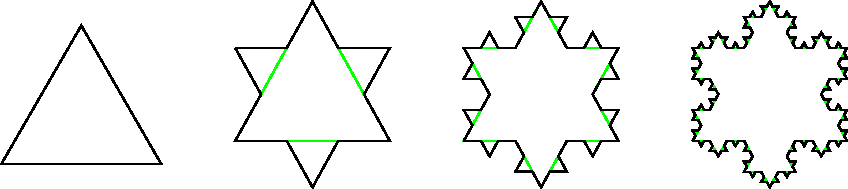
\includegraphics[width=6cm]{KochFlake.pdf} \]
Určete
\begin{enumerate}
    \item obvod $n$-té vločky,\lv{$3 \cdot \bigl(\frac43\bigr)^{n-1}$}
    \item kolik \uv{trojúhelníčků} má $n$-tá vločka navíc oproti té předchozí,\lv{$3 \cdot 4^{n-2}$}
    \item jaký obsah má navíc $n$-tá vločka oproti té předchozí,\lv{$\frac34 \cdot \bigl(\frac49\bigr)^{n-2} \cdot S$}
    \item jaký je obsah $n$-té vločky.\lv{$\frac S5 \left(8-3\bigl(\frac34\bigr)^{n-1}\right)$}
\end{enumerate}
\end{ulohav}



\baselineskip=1.25\baselineskip
\setlist[enumerate]{label=\textbf{(\alph*)},itemjoin={\quad}}

\results
\parindent=0pt
\parskip=\smallskipamount
\rightskip=0pt plus1fil\relax
\def\printvysl#1#2{\textbf{#1.} #2\par}
\vysld
\endresults


\end{document}